\part{MOTİVASYON PROBLEM TANIMI VE TEZİN AMACI}
\thispagestyle{empty}
\newpage
\section{YENİLENEBİLİR ENERJİ SİSTEMLERİNDE HABERLEŞMENİN ÖNEMİ} \label{onem}




Yenilenebilir enerji kaynaklarının dağıtık yapıda olması enerji üretim maliyetlerini arttırmaktadır. Uluslararası finansal danışmanlık ve varlık yönetimi firması olan Lazard şirketinin enerji üretim maliyet raporları incelendiğinde, bakım \& operasyon ma-liyeti olarak yaklaşık \%22 oranında rüzgar enerji santrali, ikinci sırada \%12 oranında güneş enerji santrali, üçüncü sırada yaklaşık \%10 oranında kömür termik santrali, ve son olarak \%8 oranında nükleer enerji santrali yer almaktadır.

%resim koymayı unutma

\begin{figure}[htbp]
\centerline{\includegraphics[width=\columnwidth]{Resim/chartbar.png}}
\caption{Enerji santrallerinin maliyet oranları (\protect\citeA{lazardsRapport}).}
\label{fig:Lazards}
\end{figure}

% Preamble: 





Çok etmenli yaklaşım yöntemi kullanılarak yenilenebilir enerji sistemlerinde operasyon ve bakım maliyetlerinin düşürülmesi hakkında yapılan çalışmada ancak ve ancak haberleşme sisteminin etkin bir şekilde kullanılması durumunda ilgili modelin uyarlanabilir olduğu anlaşılmıştır \cite{7804974}. 
Haberleşme sisteminin yenilenebilir enerji kaynaklarında etkin ve verimli bir şekilde kullanılması durumunda enerji üretim maliyetinin alt bileşeni olan bakım onarım ve operasyon giderlerinin maliyetlerine düşüş olacağı kaçınılmazdır.
Enerji üretim maliyetlerine doğrudan etki eden bir diğer unsur ise üretim santrallerinde yaşanan kazalardır. İlgili çalışmada güneş enerji santrallerinde haberleşme sistemine ait düzgün bir altyapının olmadığı durumlarda yaşanan kaza oranlarının daha fazla olduğu gözlemlenmiştir \cite{https://doi.org/10.1002/dac.4517}. Bu kaza durumlarının enerji üretim maliyetlerine doğru orantılı bir şekilde yansıması beklenen bir durumdur.
Mart 2022'de Uydu haberleşme hizmeti veren Euroskypark firmasına düzenlenen siber saldırı sonucu, toplamda yaklaşık 5800 adet rüzgar enerji türbininin haberleşmesi 1 saatliğine kesilmiştir \cite{sibersaldiri}. İlgili türbin topluluğunun üretim potansiyelinin 11 GW değerlerinde olduğu türbinlerin normal bir şekilde çalışmaya devam ettikleri belirtilmiştir. 11 GW'lık üretim kapasitesindeki bu türbin grubunun faaliyetlerinin 1 saatlik durması veya tamamen çalışmasına aykırı bir şekilde programlandığı durumu düşünüldüğünde yaşanabilecek sorunlar yüksek maliyet oluşturacaktır.




\section{MOTİVASYON} \label{motivasyon}



Başlık \ref{onem}'de verilen örneklerin sonucu olarak enerji üretim santrallerinin sistemli ve düzgün bir biçimde çalışması için haberleşme altyapısının doğru belirlenmesi şarttır. Bununla birlikte, yaşanacak kazaların ve problemlerin oluşturacağı maliyeti düşür-mek için kullanılan haberleşme sisteminin uygun maliyette ve uygun performans değer-lerinde olması enerji sistemleri yatırımcıları için tercih niteliği taşıyacaktır.

Bu yüksek lisans tezinde, dağıtık enerji üretim santrallerinin gerçek zamanlı olarak takibinin yapılmasına imkan sağlayacak haberleşme çözümlerinin simülasyonları tasarlanmıştır. İlgili simülasyonların performansları ve maliyetleri karşılaştırılarak, ihtiyaca göre en faydalı olacak haberleşme çözümünün belirlenmesi amaçlanmıştır.


\begin{table}[htbp]
\centering
\caption{Literatürde araştırılmış yenilenebilir enerji santrallerinin haberleşme özet tablosu}
\label{tab:literatr}

\begin{tabular}{cp{0.15\textwidth}>{\centering}p{0.12\textwidth}>{\centering}p{0.12\textwidth}>{\arraybackslash}p{0.4\textwidth}}
\hline
\\

No&\multicolumn{1}{c}{Konum}&\multicolumn{2}{c}{Haberleşme Sınıfı}&\multicolumn{1}{c}{Açıklama}\\\cline{3-4}
&&Kablolu&Kablosuz&\\

\\
\hline


1& \cite{BCIT} & Ethernet PLC &Zigbee \gls{wimax} & Üniversite kampüsüne ait 3 adet \gls{res} ve 1 adet \gls{ges} bulunmaktadır.\\
\hline

2& \cite{microgrid_siliOrnek} & Ethernet PLC & GSM & Şili'nin Atacama Çölün'de bulunan Huatacondo köyüne ait 2 adet \gls{ges} , 1 adet \gls{res} ve 1 adet dizel jeneratör sistemi bulunmaktadır.\\
\hline

3& \cite{yunanOrnek} & PLC & \gls{wifi} \gls{gsm} &Termiye Adasınaki köy evlerinin enerji ihtiyacının karşılanması için 2 MW'lık \gls{res}, 100kW'lık \gls{ges} dağıtık yapıda kurulmuştur. \\

\hline


\end{tabular}

\end{table}



Tablo \ref{tab:literatr}'de yenilenebilir enerji santrallerinde kullanılan haberleşme sistemleri hakkında yapılan çalışmaların özeti gösterilmiştir. \gls{bcit} içerisinde faal olarak çalışan yenilenebilir enerji santrallerinin akıllı şebekelere entegrasyonunda kullanılan veri haberleşme altyapısının iyileştirme projesidir \cite{BCIT}. Enstitü içerisinde 3 adet \gls{res}, 1 adet \gls{ges} bulunmaktadır. Enstitü haberleşme ağını 3 kısıma ayırmıştır. \gls{pan} kısmında Zigbee, \gls{lan} kısmında \gls{plc} son olarak \gls{wan} kısmında \gls{wimax} teknolojilerini kullanımıştır. İlgili çalışmada \gls{iec} 61850 standardı dikkate alınarak enerji santrallerinin veri modellenmesi yapılmıştır. Kullanılan veri boyutları maksimum 64 Byte civarı olarak belirlendiğinde, \gls{wimax} \%96 oranında veri iletim performansı göstermiştir. Veri boyutlarının arttırılması sonucunda paket kaybının olmadığı çalışmada gösterilmiştir. Huatacondo köyünde günlük enerji ihtiyacının \%40'lık kısmını dizel jeneratörlü enerji santralinden karşılamaktadır. Santral bünyesindeki haberleşme altyapısının performans değeri ile dizel jeneratöre olan ihtiyaç yüzdesinin ters orantılı olduğu belirtilmiştir \cite{microgrid_siliOrnek}. Ege Bölgesi'nde bulunan Termiye Adasının enerji ihtiyacı da Huatacondo köyündeki gibi hibrit enerji sistemleri üzerinden karşılanmaktadır. Adada bulunan hane sayısı ve iklim durumları göz önüne alınarak haberleşme sistemlerinin sürdürülebilir yapıda olmasına dikkat edilmiştir. Böylece Termiye Adasında dizel jeneratörlerin kullanım oranlarının düştüğü belirtilmiştir\cite{yunanOrnek}.

Akıllı şebekelerdeki \gls{lan} ağları için \gls{wifi} teknolojisi kullanılması durumunda maliyet ve sürdürülebilir yapıda haberleşmenin mümkün olduğu belirtilmiştir \cite{5779257}.

Polonya'da kurulu \gls{ges}'lere ait haberleşme altyapısının fizibilitesi ile ilgili çalışmada bulunulmuştur. Çalışmada, 4G teknolojisi uydu haberleşmeye göre daha az maliyete sahip olduğu belirtilmiştir \cite{TbarMartnez2021PositiveEO}.


Teknolojinin gelişmesiyle birlikte, daha verimli ve daha düşük bakım maliyetlerine sahip rüzgar türbinlerinin üretimi yapılmaktadır. Rüzgar türbinlerinin yönetildiği komuta kontrol merkezleri, elektrik talebine göre açılıp kapatılan rüzgar türbinlerini yönetmek ve kontrol etmekten sorumludur. İlgili makalede rüzgar türbinlerinin güç tüketimini kullanılabilirliğini ve türbin verimliliğini en üst düzeyde kontrolü için tasarlanan iletişim ağ mimarisinden bahsedilmiştir \cite{ahmed2014communication}.

2014 yılında yapılan başka bir çalışmada \cite{hussain2014multilayer} rüzgar enerjisi santralleri gerçek zamanlı izlenmesi ve kontrolü, yüksek güvenilirliğe sahip bir iletişim altyapısı gerektirdiği ile ilgili Ethernet teknolojisini SONET ortamında simülasyonu yapılmıştır.

Güneş enerji santrallerini, mevsimsel süreleri, hava durumu ve dağıtık yapıda olması gibi faktörlerden kolayca etkilenebilen bir yenilenebilir enerji sistemidir. Şebeke entegrasyonunun verimini arttırıcı faaliyetler olarak düşük gecikmeli, güvenilir ve iki yönlü iletişim esastır. Şebeke entegrasyonu için \gls{iec} 61850 standardına dayalı büyük ölçekli güneş enerji santrallerinin uzaktan izlenmesi için iletişim ağı mimarisinin tasarlanması ile ilgili çalışmalar yapılmıştır \cite{mackiewicz2006overview}.

Güneşten enerji üretimi ve sistemin kontrolü için \gls{iot} yönteminde Arduino Uno mikrodenetleyicisi ve Rasberry Pi modülleri kullanılarak enerji üretim sisteminin kontrolü ve performansının iyileştirilmesi yönünde çalışma yapılmıştır. İlgili çalışmanın topolojisi Şekil ~\ref{fig:figure3}'de gösterilmiştir \cite{deshmukh2018smart}.

\begin{figure}[htbp]
%\centerline{\includegraphics[width=7cm]{Resim/Screenshot 2022-06-12 at 20.44.42.png}}



% Gradient Info
  
\tikzset {_09use7u1u/.code = {\pgfsetadditionalshadetransform{ \pgftransformshift{\pgfpoint{-4 bp } { 0 bp }  }  \pgftransformrotate{0 }  \pgftransformscale{2 }  }}}
\pgfdeclarehorizontalshading{_s630ca86d}{150bp}{rgb(0bp)=(1,1,1);
rgb(37.5bp)=(1,1,1);
rgb(62.5bp)=(0,0,0);
rgb(100bp)=(0,0,0)}
\tikzset{_3228yxobz/.code = {\pgfsetadditionalshadetransform{\pgftransformshift{\pgfpoint{-4 bp } { 0 bp }  }  \pgftransformrotate{0 }  \pgftransformscale{2 } }}}
\pgfdeclarehorizontalshading{_7q59z2lw0} {150bp} {color(0bp)=(transparent!0);
color(37.5bp)=(transparent!0);
color(62.5bp)=(transparent!10);
color(100bp)=(transparent!10) } 
\pgfdeclarefading{_bmhgg1lnn}{\tikz \fill[shading=_7q59z2lw0,_3228yxobz] (0,0) rectangle (50bp,50bp); } 
\tikzset{every picture/.style={line width=0.75pt}} %set default line width to 0.75pt        

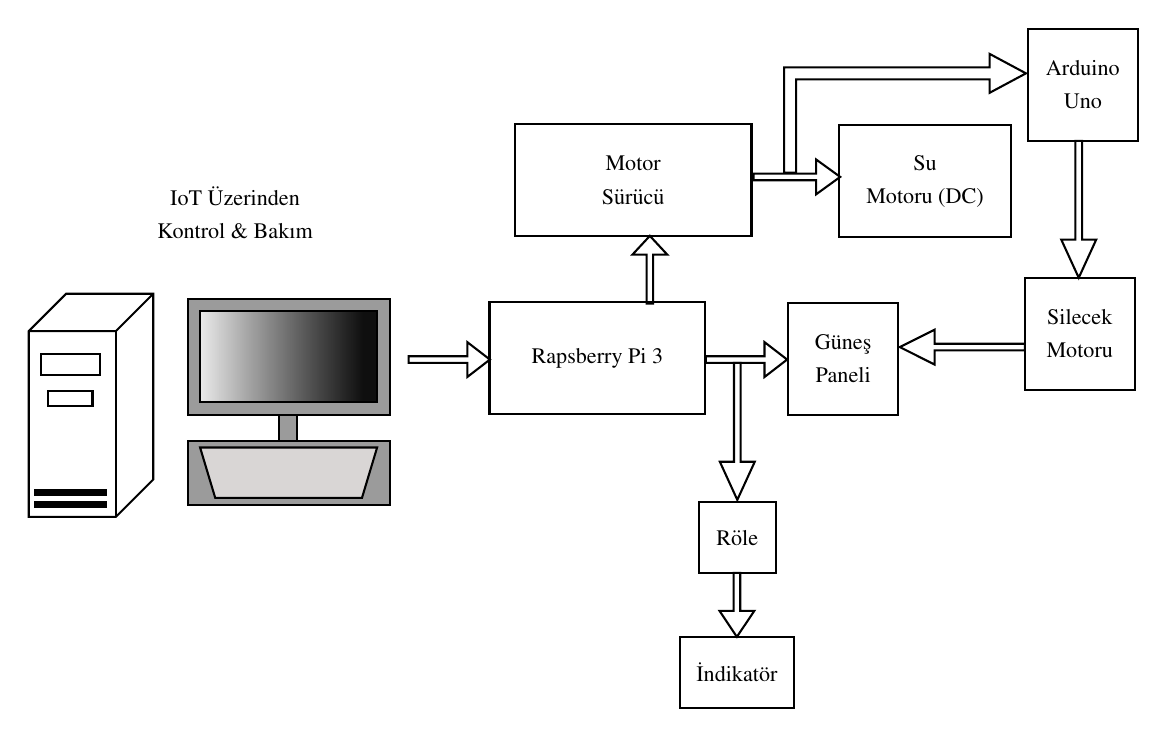
\begin{tikzpicture}[x=0.75pt,y=0.75pt,yscale=-1,xscale=1]
%uncomment if require: \path (0,426); %set diagram left start at 0, and has height of 426

%Shape: Rectangle [id:dp7780682150770082] 
\draw  [fill={rgb, 255:red, 155; green, 155; blue, 155 }  ,fill opacity=1 ][line width=0.75]  (159.1,189.62) -- (167.82,189.62) -- (167.82,206.71) -- (159.1,206.71) -- cycle ;
%Shape: Rectangle [id:dp6851387466730021] 
\draw  [fill={rgb, 255:red, 155; green, 155; blue, 155 }  ,fill opacity=1 ][line width=0.75]  (115.1,138.19) -- (212.39,138.19) -- (212.39,193.78) -- (115.1,193.78) -- cycle ;
%Shape: Cube [id:dp0343614423870906] 
\draw   (38.53,153.57) -- (56.53,135.57) -- (98.53,135.57) -- (98.53,225.07) -- (80.53,243.07) -- (38.53,243.07) -- cycle ; \draw   (98.53,135.57) -- (80.53,153.57) -- (38.53,153.57) ; \draw   (80.53,153.57) -- (80.53,243.07) ;
%Shape: Rectangle [id:dp20291484809291327] 
\draw   (44.53,164.78) -- (72.96,164.78) -- (72.96,174.5) -- (44.53,174.5) -- cycle ;
%Shape: Rectangle [id:dp031094078679610115] 
\draw   (47.96,182.35) -- (69.28,182.35) -- (69.28,189.64) -- (47.96,189.64) -- cycle ;
%Shape: Rectangle [id:dp48549901526120576] 
\draw  [fill={rgb, 255:red, 0; green, 0; blue, 0 }  ,fill opacity=1 ] (41.77,229.91) -- (75.63,229.91) -- (75.63,232.48) -- (41.77,232.48) -- cycle ;
%Shape: Rectangle [id:dp25873522519932246] 
\draw  [fill={rgb, 255:red, 0; green, 0; blue, 0 }  ,fill opacity=1 ] (41.77,235.91) -- (75.63,235.91) -- (75.63,238.48) -- (41.77,238.48) -- cycle ;
%Shape: Rectangle [id:dp8233848195769262] 
\path  [shading=_s630ca86d,_09use7u1u,path fading= _bmhgg1lnn ,fading transform={xshift=2}] (121.1,144.07) -- (206.39,144.07) -- (206.39,187.9) -- (121.1,187.9) -- cycle ; % for fading 
 \draw   (121.1,144.07) -- (206.39,144.07) -- (206.39,187.9) -- (121.1,187.9) -- cycle ; % for border 

%Shape: Rectangle [id:dp4973519926476253] 
\draw  [fill={rgb, 255:red, 155; green, 155; blue, 155 }  ,fill opacity=1 ][line width=0.75]  (115.1,206.33) -- (212.39,206.33) -- (212.39,237.21) -- (115.1,237.21) -- cycle ;
%Shape: Trapezoid [id:dp04075975469803139] 
\draw  [fill={rgb, 255:red, 217; green, 214; blue, 213 }  ,fill opacity=1 ] (121.1,209.63) -- (128.39,233.91) -- (199.1,233.91) -- (206.39,209.63) -- cycle ;
%Right Arrow [id:dp5512762508365834] 
\draw   (221.53,165.66) -- (249.84,165.66) -- (249.84,158.87) -- (260.73,167.27) -- (249.84,175.67) -- (249.84,168.87) -- (221.53,168.87) -- cycle ;
%Right Arrow [id:dp6218773129658524] 
\draw   (364.73,165.66) -- (393.04,165.66) -- (393.04,158.87) -- (403.93,167.27) -- (393.04,175.67) -- (393.04,168.87) -- (364.73,168.87) -- cycle ;
%Right Arrow [id:dp25291994634635007] 
\draw   (381.54,168.87) -- (381.54,216.52) -- (388.33,216.52) -- (379.93,234.87) -- (371.53,216.52) -- (378.33,216.52) -- (378.33,168.87) -- cycle ;
%Right Arrow [id:dp7951452337285876] 
\draw   (381.34,270.07) -- (381.34,288.32) -- (388.13,288.32) -- (379.73,300.87) -- (371.33,288.32) -- (378.13,288.32) -- (378.13,270.07) -- cycle ;
%Right Arrow [id:dp2588197140672288] 
\draw   (336.2,140.25) -- (336.2,116.72) -- (329.4,116.72) -- (337.8,107.67) -- (346.2,116.72) -- (339.4,116.72) -- (339.4,140.25) -- cycle ;
%Bend Arrow [id:dp384581087261866] 
\draw   (402.5,77.25) -- (402.5,26.51) .. controls (402.5,26.51) and (402.5,26.51) .. (402.5,26.51) -- (501.5,26.51) -- (501.5,20) -- (519,29.38) -- (501.5,38.75) -- (501.5,32.24) -- (408.23,32.24) .. controls (408.23,32.24) and (408.23,32.24) .. (408.23,32.24) -- (408.23,77.25) -- cycle ;
%Right Arrow [id:dp3009728022088294] 
\draw   (387.73,77.66) -- (417.89,77.66) -- (417.89,70.87) -- (429.5,79.27) -- (417.89,87.67) -- (417.89,80.87) -- (387.73,80.87) -- cycle ;
%Right Arrow [id:dp4821741578803411] 
\draw   (546.04,61.87) -- (546.04,109.52) -- (552.83,109.52) -- (544.43,127.87) -- (536.03,109.52) -- (542.83,109.52) -- (542.83,61.87) -- cycle ;
%Right Arrow [id:dp9449968586875006] 
\draw   (518.5,162.87) -- (474.98,162.87) -- (474.98,169.67) -- (458.23,161.27) -- (474.98,152.87) -- (474.98,159.66) -- (518.5,159.66) -- cycle ;

% Text Node
\draw (137.93,96.67) node   [align=left] {\begin{minipage}[lt]{98.6pt}\setlength\topsep{0pt}
\begin{center}
{\footnotesize {\fontfamily{ptm}\selectfont IoT Üzerinden}}\\{\footnotesize {\fontfamily{ptm}\selectfont Kontrol \& Bakım}}
\end{center}

\end{minipage}};
% Text Node
\draw    (260.53,139.47) -- (364.53,139.47) -- (364.53,193.47) -- (260.53,193.47) -- cycle  ;
\draw (312.53,166.47) node   [align=left] {\begin{minipage}[lt]{68pt}\setlength\topsep{0pt}
\begin{center}
{\footnotesize {\fontfamily{ptm}\selectfont Rapsberry Pi 3}}
\end{center}

\end{minipage}};
% Text Node
\draw    (404.43,139.87) -- (457.43,139.87) -- (457.43,193.87) -- (404.43,193.87) -- cycle  ;
\draw (430.93,166.87) node   [align=left] {\begin{minipage}[lt]{33.59pt}\setlength\topsep{0pt}
\begin{center}
{\footnotesize {\fontfamily{ptm}\selectfont Güneş}}\\{\footnotesize {\fontfamily{ptm}\selectfont Paneli}}
\end{center}

\end{minipage}};
% Text Node
\draw    (361.43,236.07) -- (398.43,236.07) -- (398.43,270.07) -- (361.43,270.07) -- cycle  ;
\draw (379.93,253.07) node   [align=left] {\begin{minipage}[lt]{22.3pt}\setlength\topsep{0pt}
\begin{center}
{\footnotesize {\fontfamily{ptm}\selectfont Röle}}
\end{center}

\end{minipage}};
% Text Node
\draw    (352.23,301.07) -- (407.23,301.07) -- (407.23,335.07) -- (352.23,335.07) -- cycle  ;
\draw (379.73,318.07) node   [align=left] {\begin{minipage}[lt]{34.82pt}\setlength\topsep{0pt}
\begin{center}
{\footnotesize {\fontfamily{ptm}\selectfont İndikatör}}
\end{center}

\end{minipage}};
% Text Node
\draw    (272.77,53.87) -- (386.77,53.87) -- (386.77,107.87) -- (272.77,107.87) -- cycle  ;
\draw (329.77,80.87) node   [align=left] {\begin{minipage}[lt]{74.66pt}\setlength\topsep{0pt}
\begin{center}
{\footnotesize {\fontfamily{ptm}\selectfont Motor}}\\{\footnotesize {\fontfamily{ptm}\selectfont Sürücü}}
\end{center}

\end{minipage}};
% Text Node
\draw    (428.87,54.37) -- (511.87,54.37) -- (511.87,108.37) -- (428.87,108.37) -- cycle  ;
\draw (470.37,81.37) node   [align=left] {\begin{minipage}[lt]{53.9pt}\setlength\topsep{0pt}
\begin{center}
{\footnotesize {\fontfamily{ptm}\selectfont Su}}\\{\footnotesize {\fontfamily{ptm}\selectfont Motoru (DC)}}
\end{center}

\end{minipage}};
% Text Node
\draw    (519.93,7.87) -- (572.93,7.87) -- (572.93,61.87) -- (519.93,61.87) -- cycle  ;
\draw (546.43,34.87) node   [align=left] {\begin{minipage}[lt]{33.59pt}\setlength\topsep{0pt}
\begin{center}
{\footnotesize {\fontfamily{ptm}\selectfont Arduino}}\\{\footnotesize {\fontfamily{ptm}\selectfont Uno}}
\end{center}

\end{minipage}};
% Text Node
\draw    (518.43,127.87) -- (571.43,127.87) -- (571.43,181.87) -- (518.43,181.87) -- cycle  ;
\draw (544.93,154.87) node   [align=left] {\begin{minipage}[lt]{33.59pt}\setlength\topsep{0pt}
\begin{center}
{\footnotesize {\fontfamily{ptm}\selectfont Silecek}}\\{\footnotesize {\fontfamily{ptm}\selectfont Motoru}}
\end{center}

\end{minipage}};


\end{tikzpicture}



\caption{Bir \gls{res}'in \gls{iot} üzerinden izlenme ve kontrolü diyagramı}
\label{fig:figure3}
\end{figure}


Dağıtım şebekelerinde \gls{wimax} ve \gls{wifi} teknolojilerinin, şebeke maliyetinde ve performansındaki durumlarını olumlu yönde etkilediği ile ilgili bir makale çalışılması yapılmış olup, Şekil ~\ref{fig:figure4}'de kurulan topoloji gösterilmiştir \cite{wlanwimaxprem}.

Yapılan çalışmada dağıtık \gls{res} ve \gls{ges}'lerde tercih edilen geleneksel haberleşme sistemlerinin dışında yenilikçi ve tamamen kapalı devre bir haberleşme sistemi kurularak \gls{ieee} ve \gls{iec} standartları ihlal edilmeden sistemin kontrolünün sağlanacağı belirtilmiştir \cite{donmezdesign}. Şekil \ref{sekildonmezmakale}'de çalışmanın topolojisi gösterilmiştir.


\begin{figure}[htbp]
\centerline{\includegraphics[width=8cm]{Resim/makaledonmez.jpg}}
\caption{\gls{ges} haberleşme topolojisi (\protect\citeA{donmezdesign}) }
\label{sekildonmezmakale}
\end{figure}

\cite{eltamaly2021iot} enerji sistemlerinde haberleşme alanında yaptığı çalışmalarda, akıllı şebekelerde kullanılan haberleşme sistemlerini inceleyip 4 katmanda toplamıştır. İlgili katmanların paket gecikme performanslarını incelemiştir.

\begin{figure}[htbp]
\centerline{\includegraphics[width=12cm]{Resim/Sekil2-3.png}}
\caption{\gls{res} haberleşme topolojisi (\protect\citeA{wlanwimaxprem}) }
\label{fig:figure4}
\end{figure}

Akıllı şebekelerin haberleşme altyapılarındaki performans değerleri simülasyon ortamında kurulup incelenmiştir. İlgili çalışmada fiber optik, \gls{wifi} ve \gls{lora} teknolojileri tek bir senaryoda sırasıyla konfigüre edilmiştir ve performans analizleri paylaşılmıştır \cite{yuan2020modeling}. 



Günümüzde rüzgar türbinleri okyanuslarda, dağlık arazilerde daha verimli bir şekilde enerji üretmektedirler. \cite{liu2010status} ilgili çalışmasında \gls{res}'lerde \gls{wimax} kullanarak performans değerlerini incelemişlerdir. Türbin sayısının artmasından kaynaklı yerleşke olarak uzak noktaların tercih edildiği rüzgar tarlalarının çalışma, üretim ve arızaların minimum gecikmeyle izlenmesi için hiyerarşik ağ yapısı yöntemiyle birden fazla komuta kontrol merkezinin haberleşme trafiğinin yönetimi ile ilgili çalışma yapılmıştır \cite{hussain2014multilayer}. Oluşturulan mimarinin gösterimi Şekil ~\ref{fig:figure6}'de paylaşılmıştır .






\begin{figure}[htbp]
\centerline{\includegraphics[width= 8 cm]{Resim/Screenshot 2022-06-12 at 21.27.08.png}}
\caption{Yenilenebilir enerji sistemlerinde hiyerarşik durum kontrol sistemi (\protect\citeA{hussain2014multilayer}) }
\label{fig:figure6}
\end{figure}

WiFi teknolojisi kullanarak Bragança Politeknik Üniversitesi kampüs alanında, güneş enerji panelinin çalışma verilerini gerçek zamanlı olarak takibi yapılmıştır \cite{delly2022solar}.
Zigbee teknolojisinin çalışma limitleri, \gls{ges}'lerin uzaktan izleme ve kontrolünde performans belirleyici unsur olarak belirtilmiştir \cite{9670354}. Dalga enerji sistemlerinin uzaktan izlenmesi hakkında yapılan çalışmada, kurulacak enerji üretim sistemindeki bileşen sayısına ve kontrol merkezinin kurulacağı noktaya göre haberleşme sisteminin belirlenmesi gerektiği belirtilmiştir \cite{johanson2019condition}.



\begin{figure}[htbp]
\centerline{\includegraphics[width= 6 cm]{Resim/Screenshot 2022-09-29 at 16.05.17.png}}
\caption{Bragança Politeknik Üniversitesi kampüs alanında kurulu çalışan prototip güneş paneli (\protect\citeA{delly2022solar}) }
\label{fig:delly}
\end{figure}



